\newpage
\subsection{Объемное планирование производства}
\label{bp:MonthPlan}

Объемное планирование производства реализовано в 1С: УПП (см. процесс ''Оперативное планирование продаж'' \ref{bp:salesplan}).

Менеджер создает документ ''Предварительная заявка'' (рис. \ref{pic:I.5.jpg}), на резервирование времени работы требуемого для изготовления заказа оборудования.

\clearpage


%Месячное планирование производства строится на основании месячного планирования продаж из отдела продаж (см. процесс ''Оперативное планирование продаж'' \ref{bp:salesplan}).

%\begin{figure}
%\begin{center}
%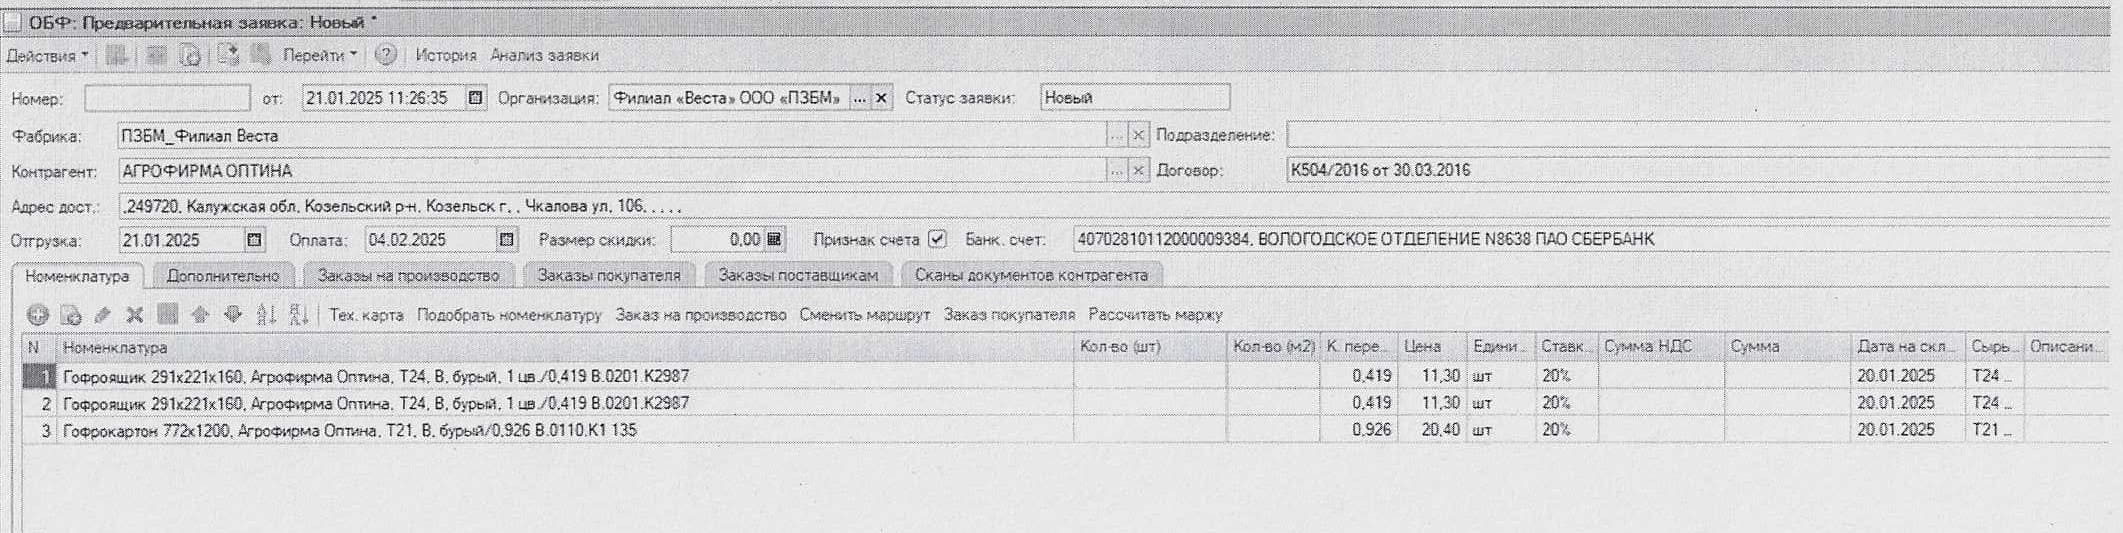
\includegraphics[height=0.17\textheight, width=1.3\textwidth, keepaspectratio]{Pics/I.5.jpg}
%\end{center}
%\caption{Форма создания предварительной заявки}
%\label{pic:I.5.jpg}
%\end{figure}
%\clearpage



% \begin{figure}
% \begin{center}
%   \includegraphics[height=0.6\textheight, angle=90, keepaspectratio]{Pics/pic_d20.jpg}
% \end{center}
%   \caption{Месячный план производства}
%   \label{pic:pic_d20}
% \end{figure}
% \clearpage


% %%
% \begin{figure}
% \begin{center}
%   \includegraphics[height=0.6\textheight, angle=90, keepaspectratio]{Pics/pic_d21.jpg}
% \end{center}
%   \caption{Месячный план с детализацией по заказам}
%   \label{pic:pic_d21}
% \end{figure}
% \clearpage


%%
%%\begin{figure}
%%\begin{center}
%%\ifnum\pdfoutput=0
%%  \includegraphics[40,0][366,292]{Pics/ProdPlan2.png}
%%\else 
%%  \includegraphics[height=0.94\textheight, keepaspectratio]{Pics/ProdPlan2.jpg}
%%\fi
%%\end{center}
%%  \caption{Месячный план производства ООО «УПП КПИ» по печатному цеху.}
%%  \label{pic:prodplan2}
%%\end{figure}
%%\clearpage
% 